\documentclass[12pt]{article}
%Gummi|065|=)
\usepackage{amsmath, amsfonts, amssymb}
\usepackage[margin=0.5in]{geometry}
\usepackage{xcolor}
\usepackage{graphicx}

\newcommand{\off}[1]{}
\DeclareMathSizes{20}{30}{20}{18}

\newcommand{\two }{\sqrt[3]{2}}
\newcommand{\four}{\sqrt[3]{4}}
\newcommand{\red}{\begin{tikz}[scale=0.25]
\draw[fill=red, color=red] (0,0)--(1,0)--(1,1)--(0,1)--cycle;\end{tikz}}
\newcommand{\blue}{\begin{tikz}[scale=0.25]
\draw[fill=blue, color=blue] (0,0)--(1,0)--(1,1)--(0,1)--cycle;\end{tikz}}
\newcommand{\green}{\begin{tikz}[scale=0.25]
\draw[fill=green, color=green] (0,0)--(1,0)--(1,1)--(0,1)--cycle;\end{tikz}}

\usepackage{tikz}

\newcommand{\susy}{{\bf Q}}
\newcommand{\RV}{{\text{R}_\text{V}}}

\title{Erdos-Szekeres Problem}
\author{John D Mangual}
\date{}
\begin{document}

\fontfamily{qag}\selectfont \fontsize{12.5}{15}\selectfont

\maketitle

\noindent One place where my nilsequences project is getting stuck is that I can't verify that certain averages form nilsequences.  
$$ n  \in \mathbb{N} \mapsto \int f(x) \; \big[f \circ T^n \big](x) \; \big[f \circ T^{2n}\big](x) \; d\mu(x)  \in \mathbb{C} $$
Logically speaking, there's a good abstact discussion showing this is true (and much more).  \\ 
This result would mean a lot more to me, if I could define a specific dynamical system $T: X \to X$ and an observable\footnote{This word ``observable" is rather loaded.  Maybe I am pushing an analogy with Quantum Mechanics?  Studying the dynamical system $T: X \to X$ is (I think) the same as studying the action of $T: L^2(X,\mu) \to L^2(X,\mu) $. \\ \\ In quantum mechanics, observables are operators (matrices) yet in our setting observables are functions.  And\dots if I really step back I think about how Ergodic Theory is meant to justify taking certain averages in Statistical Mechanics.  } $f: X \to \mathbb{R}$. \\ \\ None of the examples I can think of are terribly exciting, and dynamical systems textbooks only study a few template cases.  These experts, feel that any interesting dynamical system is ``conjugate" to a few basic cases.  \\ \\
Textbooks provide the example of the circle: $T: x \mapsto x + \sqrt{2} $ or any number $T: x \mapsto x + \alpha$ with $\alpha \notin \mathbb{Q}$. We have this dichotomy, either:
\begin{itemize}
\item $\alpha \notin \mathbb{Q}$ and $T$ is ergodic
\item $\alpha \in \mathbb{Q} $ and $T$ is \textbf{not} ergodic
\end{itemize}
So that $X = S^1 \to S^1$ and $T: X \to X$. I observe none of these rotations will be mixing, the dynamical system $T$ is simply not violent enough.  Textbooks may feel the circle example is fundamental:
\begin{itemize}
\item \dots
\item Any time we are looking prove a dynamical system is ergodic, we're looking for eigenfunctions of a unitary operators: 
$$ U_T: f(x) \in L^2(\mu) \mapsto \big[f \circ T \big] (x) \in L^2(\mu) $$
After much practice\footnote{E.g. a semseter of Quantum Mechanics} on simply knows, the eigenfunctions of unitary opeartors are the roots of unity; we are solving:
$$ \hspace{0.65in} U_T \, f = \lambda \, f \text{ and we know } \lambda = e^{2\pi i \, \alpha} \text{ with } \alpha \notin \mathbb{Q}$$ 
There is a copy of the rotation dynamical  system $T': x \mapsto x + \alpha \in S^1$ Ergodic Theory says that $\mathbf{\lambda = 1}$ is an eigenvalue. 
\end{itemize}

\newpage

\noindent We've shown that whenever we try to prove a dynamical system, the rotation $T:x \mapsto x + \alpha$ is always there.  Perhaps there will be a nil-rotation as well?  That is Terry's point.\\ \\
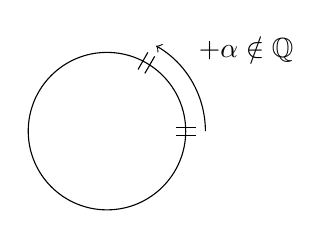
\begin{tikzpicture}
\draw (0,0) circle (1);
\draw (0.875, 0.05)--(1.125, 0.05);
\draw (0.875,-0.05)--(1.125,-0.05);
\draw (0.3941987298107782, 0.7827722283113838)--(0.5191987298107782, 0.9992785792574934);
\draw (0.48080127018922203, 0.7327722283113838)--(0.605801270189222, 0.9492785792574934);
\draw[->] (1.25,0) arc (0:60:1.25);
\node at (2.5/1.414,2.5/2.414) {$+\alpha \notin \mathbb{Q}$};
\end{tikzpicture} \\
So all dynamical systems have rotations embedded in them (either in the physical space, or the hilbert space of ``observables") by looking for eigenfunctions of 
$$  U_T : f \mapsto \big( f \circ T \big)(x) \equiv f \big[ T(x)\big] $$
If we find an eigenfunction $f$, the dynamical system restricts to a rotation:
$$  T\Big|_f : S^1 \subseteq X \to S^1 \subseteq X \text{ possibly with } \overline{S^1} = X$$
possibly this circle is dense in the entire circle. \\ \\
We could ask to quantify ergodicity: (how much) ergodic is it.  I could find irrational numbers\footnote{\texttt{https://en.wikipedia.org/wiki/Diophantine\_approximation}} $\alpha$ that are just barely outside of $\mathbb{Q}$: 
$$ \bigg| x - \frac{p}{q} \bigg| > \frac{1}{\sqrt{8} \, q^2} $$ 
There are infinitely many numbers $x \in \mathbb{Q} ``+" \frac{1}{\sqrt{8}\,q^2} $ it's hard to write this notation because the correct notation is not ``$+$".    And these kinds of rotations must also be embedding in the spectal theory of the unitary operators.  \\ \\
The real input to many of these problems will not be a dynamical systems, just a sequence of numbers $a_n \in \mathbb{R}$ (or $\mathbb{C}$) and it will our job to find a realistic $T$ (or just be OK that one might exist). \\ \\
If we found an eigenfunction $\phi$ that was invariant, we could take the Fourier coefficiets:
$$ \widehat{\phi}(n) = \int_0^1 e^{2\pi i \, k x} \phi(x) \; d\mu(x) $$
These Fourier coefficients should also be invariant under the shift map.  We could find $\widehat{\phi \circ T}(n)$:
$$ \widehat{(\phi \circ T)}(n) =\int_0^1 e^{-2\pi i \, k x} (\phi \circ T)(x) \; d\mu(x)  = e^{-2\pi i \, k \alpha } \int_0^1 e^{-2\pi i \, k x} \phi (x) \; d\mu(T^{-1}x)
= e^{-2\pi i \, k \alpha } \,\widehat{\phi}(n) $$
If $\phi$ is $T$-invariant, then $\alpha$ had better be $0$.  So there we have it $\alpha = 0$. \\ 
It could be the Fourier coefficients always agree and yet the functions are slightly different at a few points, so we use the special term $T$-\textbf{invariant almost everywhere}.
$$ \widehat{\phi}(n) = \widehat{(\phi \circ T)}(n) $$
In the case of a \textit{rotation} this means that $\hat{\phi}(n) = 0$ for $n \neq 0$. $\phi(x) = 0 + \epsilon(x)$ where $\epsilon \neq 0$ finitely many points (or a set of measure zero).

\newpage 


\noindent Thinking about it a long time, Szmeredi's theorem most helpful when a sequence of number has no good separation between structure and chance.
$$ \text{sequence} \stackrel{?}{=} \text{structure} + \text{chance} $$
and we have no idea how to separate them. This could be anything.  It defies all language.  \\ 

\begin{tikzpicture}
\draw[black!30!white] (0, 0.05)--(19, 0.05);
\draw[black!30!white] (0,-0.05)--(19,-0.05);
\end{tikzpicture} \\ 
If I choose an example from a textbook, the risk is separation is too good, and another -- must simpler -- theory could apply.\footnote{Empirical data is full of great examples of ``noise" or ``stuff" or ``garbage".  You subtract away, the best-fit-line or whatever a good Statistics textbook is telling you to do.  Try to find an explanation for what's left.  You can't.  }   Off the top of my head:
$$ T : x \mapsto 2x \pmod 1$$
This map is ergodic, it's even mixing.  Still if I am dealing with the number line, it is a little too predictible.  Maybe go a step further, I found this one after digging around:
$$ \left\{ 2^k \, 3^l\; \frac{m}{N} : 0 < k, \, l < 3 \, \log N  \right\} $$ 
I don't know which dyamical system generates these numbers, I think you need both $T: x \mapsto 2x$ and $T': x \mapsto 3x$ \dots  These numbers are $\kappa_1 (\log \log \log N)^{-\kappa_2/100} $-dense on sequenes of numbes relatively prime to $6$:  $\text{gcd}(6, N) = 1$. \\ \\
Multiplication by $\times 2$ has an entropy of $H = \log 2$ since $T^{-1}(x) = \{ 2x , 2x + 0.5\}$, so that $T^n$ should have $2^n$ pre-images. \\ \\ 
We could try it.  Let $f(x+1)=f(x)$:
$$  n \mapsto \int_0^1 f(x) \, f( 2^n x ) \, f( 2^{2n} x ) \, dx  = \mu \Bigg\{ x : 
 \big\{  x \in [0, \tfrac{1}{2}] \big\} \bigcap 
 \big\{  2^n \, x \in [0, \tfrac{1}{2}] \big\} \bigcap
 \big\{  4^n \, x \in [0, \tfrac{1}{2}] \big\} \Bigg\} $$ \\ 

\begin{tikzpicture}
\draw[black!30!white] (0, 0.05)--(19, 0.05);
\draw[black!30!white] (0,-0.05)--(19,-0.05);
\end{tikzpicture} \\ 
There must be all sorts of examples, very difficult to name just one. \\ \\
By Weyl's Law (not for free) we can count the number of lattice points inside an ellipse:
$$ \# \{ (m, n) : m^2 + \sqrt{\color{red}{2}} \, n^2 < X \} \sim \frac{X}{ 4 \times \sqrt[4]{2} } $$
I ran these numbers on my computer I found possibly that:
$$ \bigg| \# \{ (m, n) : m^2 + \sqrt{2} \, n^2 < X \} - \frac{X}{ 4 \times \sqrt[4]{2} }  \bigg| \approx { \sqrt{\color{blue}{\mathbf{2}}}} \times  \# \{ (m, n) : m^2 + \sqrt{2} \, n^2 < X \} $$
and this pattern does not hold if $\sqrt{\color{red}{2}}$ is replaced with $\sqrt{\color{red}{3}}$.  This histogram is suggestive: 

\newpage 

\includegraphics[width=3.5in]{weyl-02.png}
\includegraphics[width=3.5in]{weyl-01.png} \\

\noindent I can't the center is exactly $\sqrt{2}$ and the pattern breaks down for other values of $\alpha$, but there's some clear convergence and there's a split between values above and below the line.   \\ \\
We could ask how many values of $(m,n)$ lie significantly above or below the median. 
$$ f(X) =  \# \{ (m, n) : m^2 + \sqrt{2} \, n^2 < X \} \text{ when does }
\left|f(x) -   \frac{\pi}{4 \times \sqrt[4]{2} } X \right| \stackrel{?}{>} c \times \sqrt{X} $$
I think a reasonable number is $c = 2$.  This is the idea $f(X)$ is impossible to calculate exactly for all value, we find average that looks pretty good, most of the time. \\ \\
That just becomes our starting point to look for exceptions.  These ``obvious" statements can be a nuisiance to prove, maybe because we underestimate how much information lies in there. \\ \\
Step back a minute, we are counting lattice points inside of a circle:
$$ \# \{ (m,n):  m^2 + n^2 < X \} \approx \pi X $$
This is known as the \textbf{Gauss circle problem} and we know that 
$$ \# \{ (m,n):  m^2 + n^2 < X \}  =  \pi X  + O(X) \text{ maybe } \stackrel{?}{=}\pi X + O(\sqrt{X})$$
which is what I'm observing on my computer. \\ \\
This problem is hard, therefore must be a lot of ``information".  These signals are of a rather difficult and unknown nature.  This may be a candidate for Terry's nilsequence techiques.

\vfill

\begin{thebibliography}{}

\item Alexander Leibman \\ \textbf{Nilsequences, null-sequences, and multiple correlation sequences} \texttt{ arXiv:1205.4004} 
\item 
Terry Tao \\
\texttt{https://terrytao.wordpress.com/2017/04/28/notes-on-nilcharacters-and-their-symbols/}
\texttt{https://terrytao.wordpress.com/2017/05/05/} ( New bounds for Szemer\'{e}di's theorem, III )

\item Luis Barreira \\ \textbf{Ergodic Theory, Hyperbolic
Dynamics and Dimension
Theory} (Univertext) Springer, 2012. \\ 
Manfred Einsiedler, Thomas Ward \\ \textbf{Ergodic Theory
with a view towards Number Theory} (GTM, \# 259) Springer, 2011.

\item Jean Bourgain, Elon Lindenstrauss, Philippe Michel, Akshay Venatesh. \textbf{Some effective results for $\times a \times b$} Ergodic theory and dynamical systems (2009).

\item Valentin Blomer, Jean Bourgain, Maksym Radziwi\l\l, Zeev Rudnick \textbf{Small gaps in the spectrum of the rectangular billiard} \texttt{arXiv:1604.02413}

\end{thebibliography}


\newpage

\noindent The candidate I have for ``naturally occuring" dynamical systems.\footnote{The fact that Artur Avila is studying the Thousless Transition points could have a nice tie-in to the 2016 Nobel Prize in Physics.  Not 100\% sure if the names are correct, or if I have a mix-up.}  Mostly they are Hamiltonians of physical dynamical systems:
$$ \boxed{\text{let }T = H} $$
Mostly, any physics textbook problem is either an embedded copy of a rotation or a harmonic oscillator:
\begin{itemize}
\item a spring (or a swing)
\item a spinning top
\end{itemize}
All of classical mechanics amounts to finding embedded copies of these two physical systems in nature\dots 
\begin{itemize}
\item We can evolve a small region of phase space and it get's really stretchy and twisty
\item We can find an easy solution and study the space of solutions ``nearby"
\end{itemize}
The team of three, choose a Hamiltonian to study, not the easiest to write down
$$ (H_{\theta; \lambda, \alpha })_k 
= v(\theta +  \alpha k) \psi_k 
+ c_\lambda (\theta + \alpha k) \psi_{k+1} + 
\overline{c_\lambda (\theta + a(k-1)) } \psi_{k-1}  $$
where $c_\lambda$ and $v$ are two numbers:
$$c_\lambda = \lambda_1 e^{-2\pi i \, \theta + \frac{\alpha}{2}}  + \lambda_2 + \lambda_3 e^{2\pi i \, \theta + \frac{\alpha}{2}} \quad v(\theta ) = 2 \cos (2\pi \theta) $$
This operator is rather complicated.  Lots of literature written about it in 1980's but maybe as thorough discussio as Avila is about to give.\footnote{and maybe Physicists did not really care about  such trivialities as ``convergence" and ``Lyapounov exponents"} \\ \\
We have gone the opposite extreme already.  I have no chance of obtaining the nilsequence averages I wanted on the first page.  Instead he moves in an entirely different direction. 
$$ \liminf_{n \to \infty} \max_{|z|=1} \prod_{k=1}^n \big|z - e^{2\pi i \, k \alpha } \big| \stackrel{?}{<} \infty  $$
and then I obtained this function in a different way using numerical approximation.
$$ f \big (\Delta t \big) = \sum_{k=0}^{\frac{1}{\Delta t}} \sin \big( 2\pi k \, \Delta t \big) $$
And as the mesh shrings to zero, $||\Delta t|| \to 0$, the Riemann sums ``bounce" very much like the funtion Avila describes.  \\ \\
Continued fractions (or more complicated objects) seem to be describing how are ``approximate" solutions to differential equations are failig.  \\ \\
As it stands, I think we can get the nilsequences by studying interesting sequeneces of numbers and comparing them to the textbook dynamical systms such as the shift map or horocycle flow.



\begin{thebibliography}{}

\item Mei-Chu Chang, Jean Bourgain \textbf{On a paper of Erd\"{o}s and Szekeres} \texttt{arXiv:1509.08411}

\item Artur Avila, Svetlana Jitomirskaya, C. A. Marx \textbf{Spectral theory of extended Harper's model and a question by Erd\"{o}s and Szekeres} \texttt{arXiv:1602.05111} 

\item Artur Avila, Svetlana Jitomirskaya, Qi Zhou \textbf{Second Phase transition line} \texttt{arXiv:1608.01799} 

\item Amie Wilkinson \textbf{What are Lyapunov exponents, and why are they interesting?} \texttt{arXiv:1608.02843} 

\newpage

\noindent Foliations and continued fractions seem to emerge in the \textbf{perturbation theory} of physical systems.\footnote{our vauge and abstract language means we have no idea what we're talking about :-)  If we want, we can find a situation where KAM theory does't exist, and maybe our generalized continued fraction object will be there!  Our textbooks only show the cases where perturbation theory behaves nicely\dots } With our shallow understanding about why number theory might be relavant to classical mechanics, we go back to textbook problems.  \\ \\
Mainly, if we deviate from eqilibrium solutions (or from cycles) or change our dyamical system slightly, the orbts will get very complicated again.  There are tools:
\begin{itemize}
\item Kolomogorov-Arnold-Moser theory
\item Aubry-Mather theory
\end{itemize}
Maybe the word I am missing is ``tractable".  There are always dynamical systems, very few I can say anything intelligent about. \\ \\
Here's maybe a way to get realistic nilsequences:
\begin{itemize}
\item I want to show that Gaussian primes (in $\mathbb{Z}[i]$) are rotationally symmetric
\item I will find a modular form and show that since the horocycle flow is mixing,
we can obtain a really good estimate of the coefficients.  
\item the error terms to equidistribution (or mixing) will have some faint noise that never goes away.
\end{itemize}
There are lots and lots of modular forms, and lots of instances of the horocycle flow, but I knew of a limited few exmples where the Ratner theory matches up with a Diophantine Equation. 
\vfill

\begin{thebibliography}{}

\item Etienne Ghys \textbf{R\'{e}sonances et petits diviseurs}, Colloque ``Fourier", Auxerre 2002, publi\'{e} dans la deuxi\`{e}me \'{e}dition de ``L'h\'{e}ritage de Kolmogorov", Belin. Traduction anglaise dans ``Kolmogorov's heritage in mathematics", 187-213, Springer, Berlin, 2007.  \\ \\
\texttt{http://perso.ens-lyon.fr/ghys/articles/resonancesmall.pdf}
\texttt{http://perso.ens-lyon.fr/ghys/articles/resonancesdiviseurs.pdf}


\end{thebibliography}

\end{thebibliography}

\end{document}